\documentclass[10pt]{beamer}
\usefonttheme{professionalfonts,serif}
\def\newblock{\hskip .11em plus .33em minus .07em}
\usepackage[numbers,sort]{natbib}
\renewcommand{\rmdefault}{psbx}
\usepackage[utf8]{inputenc}
\usepackage[T1]{fontenc}
\usepackage{textcomp}
\usepackage{eulervm}

\usetheme{default}           % tips from David Blei
\useinnertheme{circles}
\useoutertheme{infolines}
\setbeamertemplate{headline}{}
\setbeamertemplate{navigation symbols}{}
\setbeamerfont{itemize/enumerate subbody}{size=\normalsize}
\setbeamerfont{itemize/enumerate subsubbody}{size=\normalsize}
\usecolortheme{seahorse}
\setbeamersize{text margin left=2mm,text margin right=2mm}

\graphicspath{{../../figures/}}

\definecolor{mypine}{rgb}{0.05,0.45,0.05}
\definecolor{mycyan}{rgb}{0.0,0.9,0.9}
\newcommand{\Red}{\textcolor{red}}
\newcommand{\Blue}{\textcolor{blue}}
\newcommand{\Green}{\textcolor{mypine}}
\newcommand{\PineGreen}{\textcolor{mypine}}
\newcommand{\Magenta}{\textcolor{magenta}}
\newcommand{\Cyan}{\textcolor{mycyan}}

\newcommand{\N}{\mathcal{N}}
\newcommand{\R}{\mathbb{R}}
\newcommand{\T}{{\scriptsize^{\top}}}
\newcommand{\D}{\mathcal{D}}
\newcommand{\F}{\mathcal{F}}
\newcommand{\E}{\mathbb{E}}
\newcommand{\V}{\mathbb{V}}
\newcommand{\M}{\mathcal{M}}
\newcommand{\KL}{\mathcal{KL}}
\newcommand{\cut}[1]{}
\newcommand{\trace}{\operatorname{trace}}

\newcommand{\bmu}{{\boldsymbol{\mu}}}
\newcommand{\btheta}{\boldsymbol{\theta}}
\newcommand{\bepsilon}{\boldsymbol{\epsilon}}
\newcommand{\balpha}{\boldsymbol{\alpha}}
\newcommand{\bbeta}{\boldsymbol{\beta}}
\newcommand{\bphi}{\boldsymbol{\phi}}
\newcommand{\bPhi}{\boldsymbol{\Phi}}
\newcommand{\bSigma}{\boldsymbol{\Sigma}}
\newcommand{\bpi}{\boldsymbol{\pi}}
\newcommand{\blambda}{\boldsymbol{\lambda}}

\newcommand{\argmax}{\operatorname{argmax}}
\newcommand{\argmin}{\operatorname{argmin}}
\newcommand{\ci}{{\bot\negthickspace\negthickspace\bot}} % conditional indep.
\newcommand{\neigh}{\operatorname{ne}}
\newcommand{\vectr}[2]{  \left[ \!\!\begin{array}{c} #1 \\
      #2 \end{array} \!\!\right]}
\newcommand{\deff}{\stackrel{\mathrm{def}}{=}}
\newcommand{\deldel}[2]{\frac{\partial #1}{\partial #2}}

\newcommand{\maketilde}{\raisebox{0.4ex}{\tiny $\sim$}}
\newcommand{\bfa}{\mathbf a}
\newcommand{\bfb}{\mathbf b}
\newcommand{\bfe}{\mathbf e}
\newcommand{\bff}{\mathbf f}
\newcommand{\bfk}{\mathbf k}
\newcommand{\bfm}{\mathbf m}
\newcommand{\bfn}{\mathbf n}
\newcommand{\bfp}{\mathbf{p}}
\newcommand{\bfs}{\mathbf s}
\newcommand{\bfu}{\mathbf u}
\newcommand{\bfx}{\mathbf x}
\newcommand{\bfy}{\mathbf y}
\newcommand{\bft}{\mathbf t}
\newcommand{\bfv}{\mathbf v}
\newcommand{\bfw}{\mathbf w}
\newcommand{\bfA}{\mathbf A}
\newcommand{\bfI}{\mathbf I}
\newcommand{\bfK}{\mathbf K}


\title{Gibbs Sampling for Bayesian Mixture}
\author{Carl Edward Rasmussen}
\date{November 25th, 2016}

\begin{document}


\begin{frame}
\titlepage
\end{frame}


\begin{frame}
\frametitle{Key concepts}

\begin{itemize}
\item General Bayesian mixture model
\item We derive the Gibbs sampler
\item Marginalize out mixing proportions: collapsed Gibbs sampler
\end{itemize}

\end{frame}


\begin{frame}
\frametitle{Bayesian mixture model}

A mixture model has observations ${\bf y}$, parameters
$\boldsymbol\beta$, and latent variables ${\bf z}$.\\[1ex]

There are $N$ observations, $y_n, n=1,\ldots N$. The mixture model has $K$
components, so the parameters are $\beta_k, k=1,\ldots K$ with prior
$p(\boldsymbol\beta)$ and the
discrete latent variables $z_n, n=1,\ldots N$ take on values $1,\dots
K$.\\[1ex]

The Bayesian mixture of categoricals is an example (although in this
case, the observations are the $D$ documents).

\begin{minipage}{0.7\linewidth}
\centerline{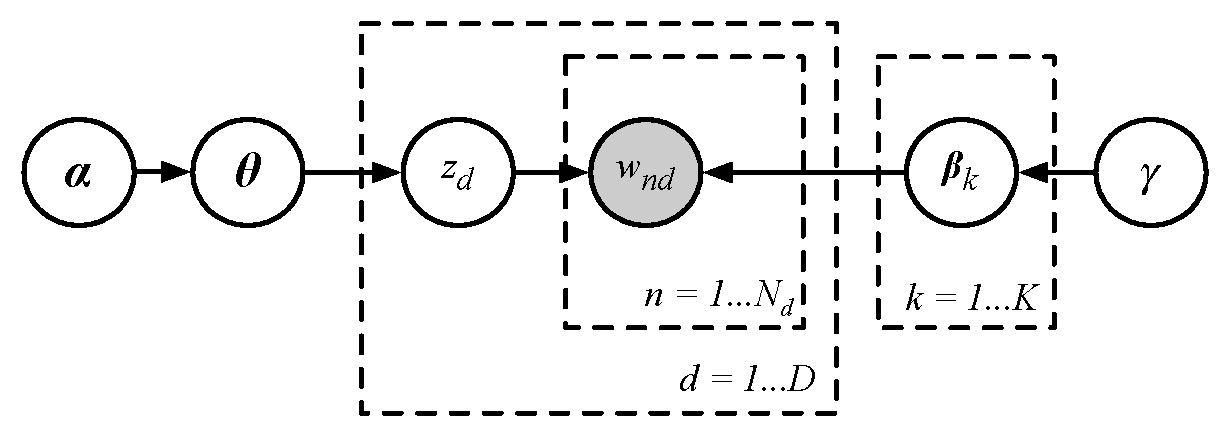
\includegraphics[width=0.9\linewidth]{bayes_mix_categorical_model}}
\end{minipage}
\begin{minipage}{0.29\linewidth}
{\small
\begin{eqnarray*}
\btheta & \sim & \mathrm{Dir}(\alpha) \\
\bbeta_k & \sim & \mathrm{Dir}(\gamma) \\
z_d | \btheta & \sim & \rm{Cat}(\btheta)\\
w_{nd} | z_d, \bbeta & \sim & \rm{Cat}(\bbeta_{z_d})
\end{eqnarray*}
}
\end{minipage}
\end{frame}



\begin{frame}
\frametitle{Bayesian mixture model}

The conditional likelihood is for each observation is
\[
p(y_n|z_n=k,\boldsymbol\beta)\;=\;p(y_n|\beta_k)\;=\;p(y_n|\beta_{z_n}),
\]
and the prior
\[
p(\boldsymbol\beta_k).
\]

The categorical latent component assignment probability
\[
p(z_n=k|\boldsymbol\theta)\;=\;\theta_k,
\]
with a Dirichlet prior
\[
p(\theta|\alpha)\;=\;{\rm Dir}(\alpha).
\]

Therefore, the latent posterior is
\[
p(z_n=k|y_n,\boldsymbol\theta,\boldsymbol\beta)\;\propto
p(z_n=k|\boldsymbol\theta)p(y_n|z_n=k,\boldsymbol\beta)\;\propto\;
\theta_k p(y_n|\beta_{z_n}),
\]
which is just a discrete distribution with $K$ possible outcomes.
\end{frame}


\begin{frame}
\frametitle{Gibbs Sampling}

Iteratively, alternately, sample the three types of variables:\\[1ex]

Component parameters
\[
p(\beta_k|{\bf y},{\bf z})\;\propto\;p(\beta_k)\prod_{n:z_n=k}p(y_n|\beta_k),
\]
which is now just a regular model, the mixture aspect having been eliminated.\\[1ex]

The latent allocations
\[
p(z_n=k|y_n,\boldsymbol\theta,\boldsymbol\beta)\;\propto \theta_k
p(y_n|\beta_{z_n}),
\]
and mixing proportions
\[
p(\theta|{\bf z},\alpha)\;=\;p(\theta|\alpha)p({\bf z}|\theta)\;=\;
{\rm Dir}(\frac{c_k+\alpha_k}{\sum_{j=1}^K c_j+\alpha_j}).
\]
where $c_k=\sum_{n:z_n=k}1$ are the counts for mixture $k$.
\end{frame}

\begin{frame}
\frametitle{Collapsed Gibbs Sampler}

The parameters are treated in the same way as before.\\[1ex]

If we \Blue{marginalize} over $\theta$
\[
p(z_n=k|{\bf z}_{-n},\alpha)\;=\;\frac{\alpha+c_{-n,k}}{\sum_{j=1}^K\alpha+c_{-n,j}},
\]
where index $-n$ means \emph{all except} $n$, and $c_k$ are counts;\\
we derived this result when discussing pseudo counts.\\[1ex]

The \Blue{collapsed} Gibbs sampler for the latent assignements
\[
p(z_n=k|y_n,z_{-n},\boldsymbol\beta,\alpha)\;\propto
p(y_n|\beta_k)\frac{\alpha+c_{-n,k}}{\sum_{j=1}^K\alpha+c_{-n,j}},
\]
where now all the $z_n$ variables have become \Blue{dependent} (previously
they were conditionally independent given $\theta$).\\[1ex]

Notice, that the Gibbs sampler exhibits the \emph{rich get richer} property.
\end{frame}
\end{document}
